\subsection{Placement of edge data centres \emph{Ericsson}}
\subsubsection{Proposed research}
There are no clear directions as to what degree the coming mobile networks will be virtualized. The degree of virtualization will determine the distribution of compute resources in the network, bounded by properties such as propagation delay, and cell resource provisioning.

The geographic domain in which users move, the location and size of the \xcloud hosting entity defines the bounds in which the service can perform optimally.

We propose a service performance study into the placement of the \xcloud resources. The study will contrast the service delay performance with the placement of the \xcloud resources ranging from the radio bases station to the adjacent core network, where there the \xcloud node caters for multiple base stations.

\begin{figure}
	\centering
	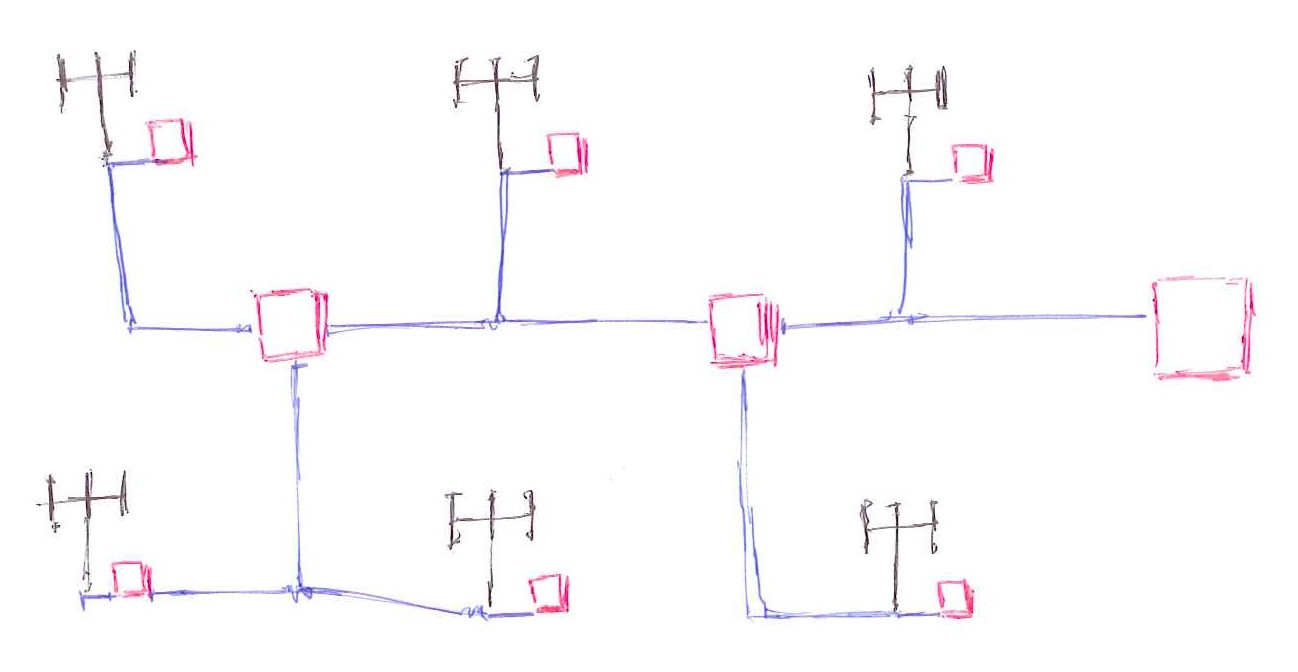
\includegraphics[width=\linewidth]{placement_diagram.jpg}
	\caption{\xcloud placement}
	\label{diagram_placement}
\end{figure}

The service delay will be determined by the additive latency in the mobile network, the level of congestion in the \xcloud node, and the resource shift instigated by user mobility.

We propose to contract the latency experienced by the user with the additional load imposed on the \xcloud infrastructure, as a form of utility.
\subsubsection{Related research}